This chapter describes the design and implementation of the core translation memory. The core translation memory is the part of the project that is responsible for retrieving and ranking suitable suggestions for chunks in the subtitle file that the user is translating.

\section{Preliminaries}

\subsection{Choosing a DBMS}
\label{sec:dbms}

For the choice of a suitable database management system underlying the
core translation memory and the user space, the main points we
considered were

\begin{itemize}
\item
  software license of the DBMS
\item
  general performance and maintainability
\item
  included support for fuzzy matching and custom indexes
\end{itemize}
According to these requirements, we evaluated several database systems
and selected the open source database system
\postgres.\footnote{\url{http://www.postgresql.org/}, written either Postgres or PostgreSQL} This system
fulfills the requirements as follows:

\begin{itemize}
\item
  open license similar to BSD license
\item
  good results in performance evaluations and good reputation for
  maintainability
\item
  support for phonetic representation of strings (SOUNDEX and
  METAPHONE), string edit distance (Levenshtein), fuzzy string search
  using character trigrams and customizable indexes (GIST, GIN)
\end{itemize}

For managing connections to the database in Java and Scala, we use JDBC, 
which allows the database connection to easily use another DBMS. 
In the XML-based configuration file (see the installation manual, Chapter~\ref{chap:technical_manual}), the JDBC connector
and username and password to the database have to be specified. When testing the
translation memory with project-internal unit tests, we replace the production JDBC
configuration with a temporary in-memory database (HSQLDB\footnote{\url{http://hsqldb.org/}}).

\lstset{language=XML, caption={Configuration snippet}}
\begin{lstlisting}
<database>
    <connector>jdbc:postgresql://localhost/filmtit</connector>
    <user>postgres</user>
    <password>postgres</password>
</database>
\end{lstlisting}


\subsection{Retrieving Media Source Information}

For retrieving information about media sources, we initially used a free IMDB API (\url{http://imdbapi.com/}). However, it showed that this API might become unreliable in the future and indeed, as of July 30, the API had been shut down. To avoid complications early, we switched to the Freebase API\footnote{\url{http://www.freebase.com/}}. Freebase is a large knowledge base of structured data based on data extracted from Wikipedia and other publicly available resources and continually extended by users.

To retrieve media source candidates, first a full text search query with the title and a restriction to entities of type \emph{film}\footnote{Freebase type: /film/film.} and \emph{TV program}\footnote{Freebase type: /tv/tv\_program.} is sent to the Freebase API. Afterwards additional information for each candidate is retrieved and the {\tt MediaSource} objects are sent to the GUI for the best match to be selected by the user.



\section{Architecture of the Core Translation Memory}
\label{sec:corearchitecture}

The core translation memory consists of the database of chunks and media
sources (movies and TV shows) which are indexed in several ways for fast
retrieval. A query to the translation memory generally proceeds in two
steps: In a first step, translation pairs for a chunk are retrieved from
the database. The second step consists of ranking the candidates
retrieved in the first step according to their quality and how well they
match the query. If the quality of the retrieved candidates exceeds a
minimum quality threshold, they will be sent to the user.

\subsection{Backoff Translation Memories}

The idea of a backoff translation memory is to use multiple ways of
retrieving and ranking candidate translation pairs from the database and
``back off'' to a less exact level of retrieval and ranking when there
are no satisfying results on the current level.

A backoff-level in the translation memory consists of a \emph{translation pair
searcher}, a \emph{translation pair ranker} and a \emph{minimal quality
threshold}. 
If the results retrieved by the \emph{searcher} and scored and ranked by
the \emph{ranker} do not meet the threshold, then the query is sent to the 
next level of the backoff translation memory. 


\section{Candidate Retrieval}
\label{sec:candidate_retrieval}

We implemented several methods for efficiently retrieving candidate
translation pairs from the database. 


\subsection{Translation Pair Searchers}

Every translation pair searcher implements the interface {\tt TranslationPairSearcher} and therefore must implement the method 

\vspace*{0.5em}

\lstset{language=scala, caption={Candidate search}}
\begin{lstlisting}
def candidates(chunk: Chunk, language: Language): List[TranslationPair]
\end{lstlisting}

This is the main method for retrieving translations pairs, which are then combined and ranked in later steps. A {\tt TranslationPairSearcher} may require the chunks it queries to be tokenized beforehand. In this case, the {\tt TranslationPairSearcher} must override the following method:

\vspace*{0.5em}

\lstset{language=scala, caption={TranslationPairSearchers may require tokenization}}
\begin{lstlisting}
def requiresTokenization: Boolean
\end{lstlisting}

\vspace*{0.5em}



{\tt TranslationPairSearcher}s that are based on the local \postgres~database extend the class {\tt TranslationPairStorage} and must implement the method {\tt add} for adding new translation pairs to the storage.

\vspace*{0.5em}
 
\lstset{language=scala, caption={TranslationPairSearchers may require tokenization}}
\begin{lstlisting}
def add(translationPairs: TraversableOnce[TranslationPair])
\end{lstlisting}

\vspace*{0.5em}


The method {\tt reindex} must be implemented to create and update the database indexes for the particular searcher.

\lstset{language=scala, caption={TranslationPairSearchers may require tokenization}}
\begin{lstlisting}
def reindex()
\end{lstlisting}








\subsection{Tokenization}
\label{sec:tokenization}

For all program-based retrieval methods, we tokenize, i.e.\ separate the input sentence into individual tokens,
all inputs, using tokenizers provided by the Apache OpenNLP project.\footnote{\url{http://opennlp.apache.org/}}
OpenNLP provides both unsupervised and supervised methods of tokenization. 
As a default tokenizer, we use an unsupervised tokenizer that splits the input
based on whitespace. This method has the advantage that it is applicable to any new
language without requiring further training, however the result is of moderate
quality and often leads to problems in latter processing steps (e.g. Named Entity Recognition).

To improve the results, we use a Maximum-Entropy based OpenNLP tokenizer. For English, we use the
models provided by the OpenNLP project. 


\subsubsection*{Czech ME tokenizer}

For Czech, no such model existed, so we trained a ME tokenizer
model on data from the Prague Dependency Treebank\footnote{\url{http://ufal.mff.cuni.cz/pdt2.0/}}. Scheme of the process is in fogure \ref{fig:tokenizer}. 

We produced a script that creates training data in the following format:
\begin{verbatim}
K vynikajícím spisovatelům<SPLIT>, kteří věřili v nevysvětlitelné duševní 
úkazy<SPLIT>, patřil také americký romanopisec Upton Sinclair<SPLIT>.
\end{verbatim}

\begin{figure}[h]
\begin{center}
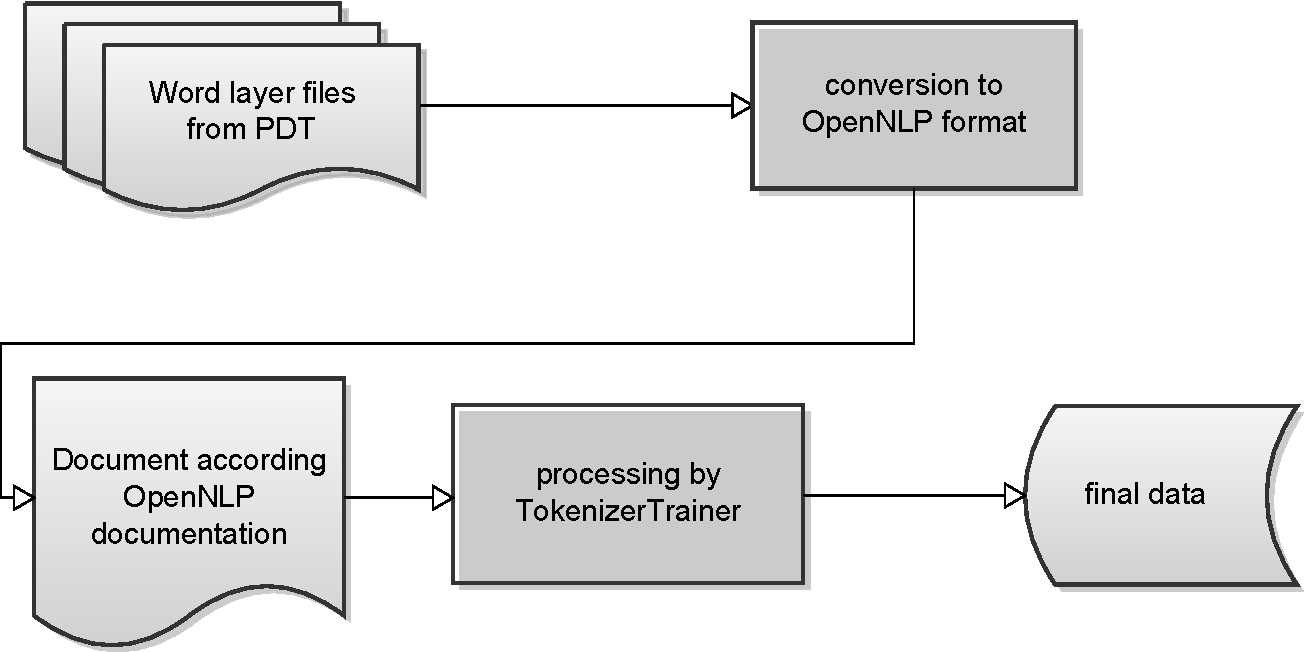
\includegraphics[scale=0.6]{figures/creatingTokenizationModel.pdf}
\end{center}
\caption{Scheme of traning the tokenizer.}
\label{fig:tokenizer}
\end{figure}

In the training data, the \verb|<SPLIT>| annotation indicates a position in the data, in which the
tokenizer is required to separate two tokens (in this case words and punctuation symbols). These
positions were manually marked in the Prague Dependency Treebank by annotators.

On a test dataset from the Prague Dependency Treebank, the ME tokenizer achieved the following results:

\lstset{caption={Accuracy for the Czech ME tokenizer.}}
\begin{lstlisting}
Precision: 0.9970180340649772
Recall: 0.9954658318039512
F-Measure: 0.9962413283293529
\end{lstlisting}


\subsection{Signature-Based Retrieval}

The most general method is the usage of indexed signature strings. There are two implementations of signature-based retrieval in the project: In the first method, signatures are created fully within the \postgres~database (database-based signatures) and in the second, the signatures are created on the server and only stored and retrieved in the
database (program-based signatures).  


\subsubsection*{Program-based signatures}

In the case of program-based signatures, for each chunk stored in the database, a string is produced by a signature function and this string is used to retrieve candidates from a signature table that is in turn
connected to the translation pairs table.

\begin{figure}[h!]
	\centering
		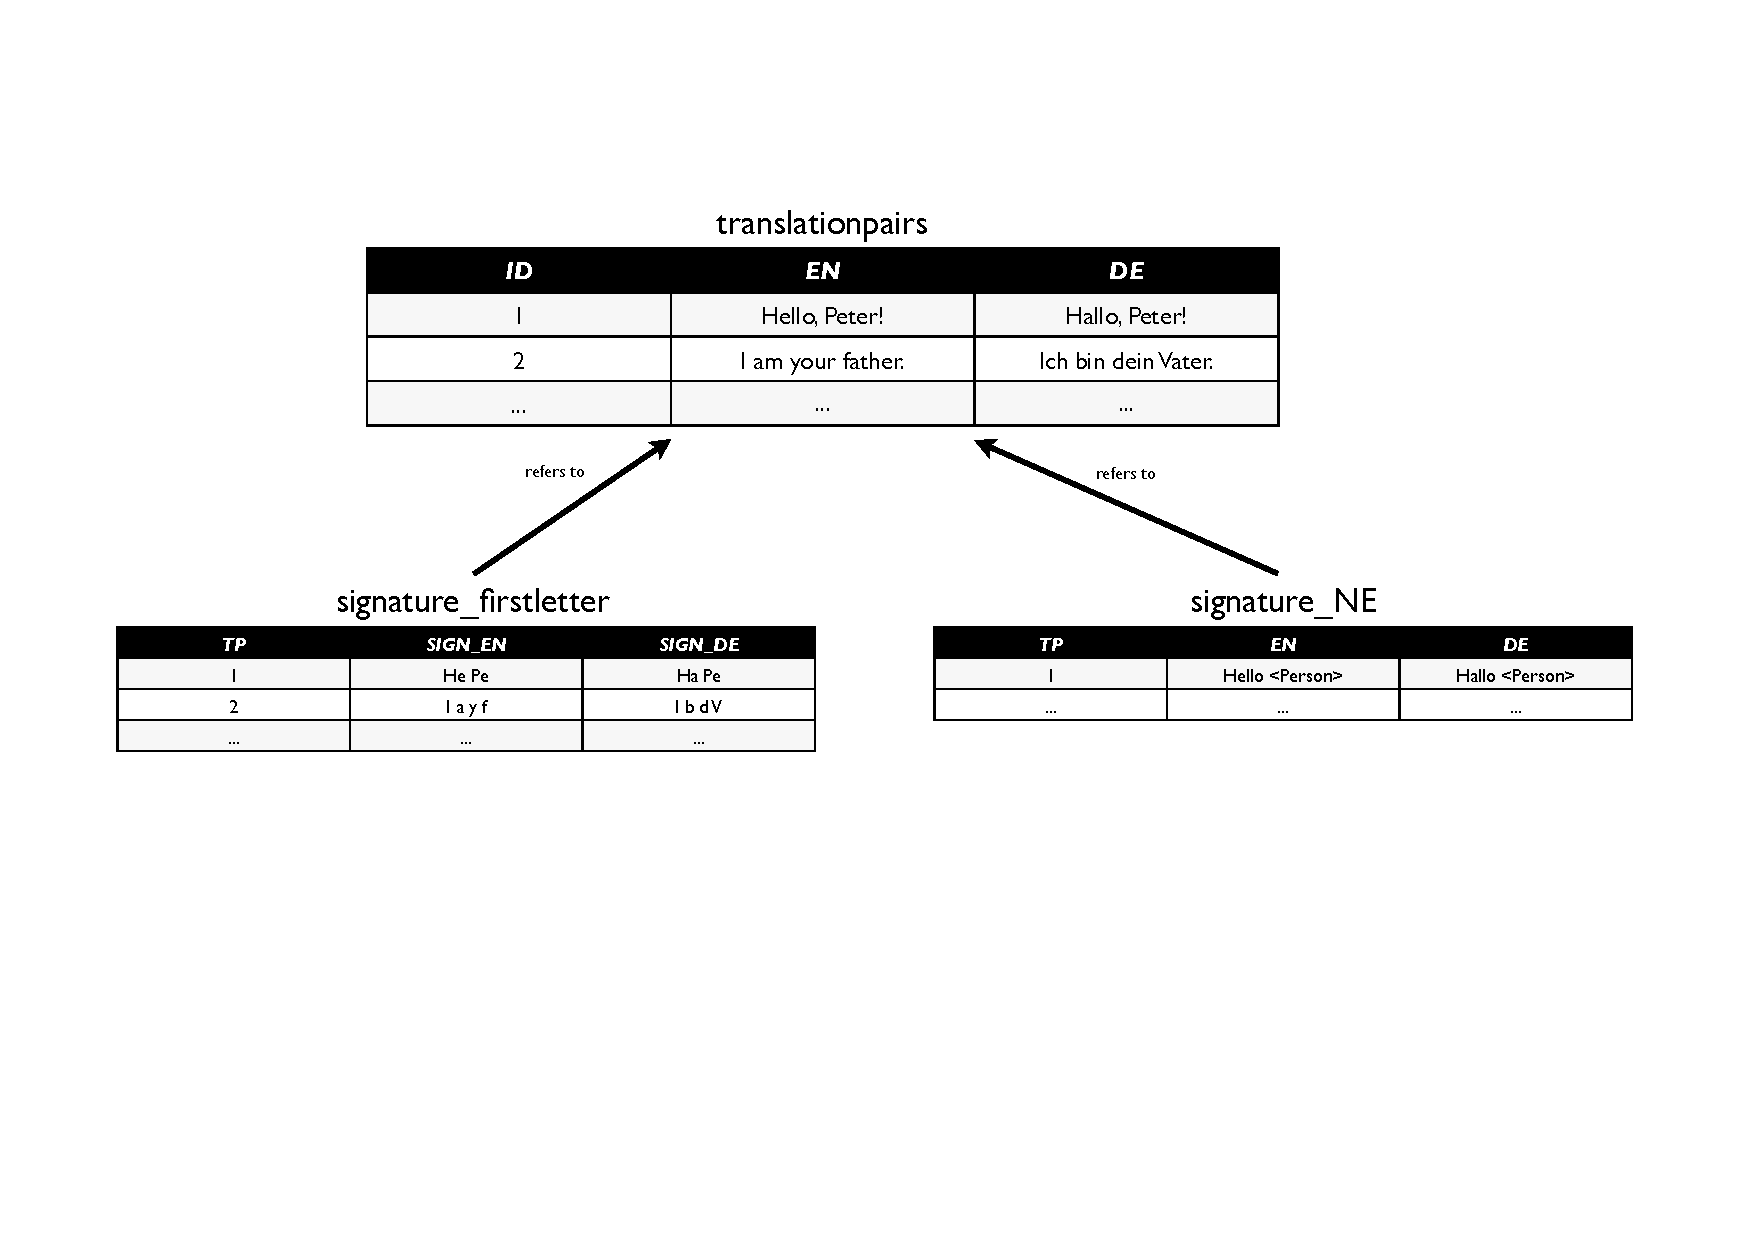
\includegraphics[width=17cm]{figures/core/signatures.pdf}
	\caption{Illustration of signature strings in the database.}
	\label{fig:figures_core_signatures}
\end{figure}


\subsubsection*{Database-based signatures}

In the case of the database-based signatures, a {\tt PL/pgSQL} procedural function is used to create a functional index\footnote{See e.g.\ \url{http://www.postgresql.org/docs/9.1/static/indexes-expressional.html} (retrieved 02.08.2012).} on the translationpairs table. The function can then be used for fast retrieval from this table.


Several signature functions are used in the translation memory
implementation. In the following sections, the signature functions and related issues will be illustrated.


\subsection{Signature-Based Retrieval: Exact Matches}

The first signature function is for retrieving exact matches. For this,
the signature function consists of the first letters of each word in the
chunk. Punctuation is dropped from the signature. If the queried chunk is
short, only using the first letter would produce a very high number of
results. Hence, for short chunks, more letters of each individual token are
included. Algorithm~\ref{alg:firstletter} shows pseudo-code for the {\tt FirstLetter}
function.

\vspace{1em}
\begin{algorithm}[H]
\label{alg:firstletter}
 \SetKwFunction{Union}{Union}\SetKwFunction{TokenizeAndRemoveStopWords}{TokenizeAndRemoveStopWords}
 \SetKwFunction{Union}{Union}\SetKwFunction{Lower}{Lower}
 \SetKwFunction{Union}{Union}\SetKwFunction{Take}{Take}


 \SetAlgoLined

 \KwData{text chunk}
 \KwResult{signature for the chunk}
 $tokens \leftarrow \TokenizeAndRemoveStopWords{chunk}$

 \For{$token \in tokens$}{

   \uIf{$|token| = 1$}{
     ret += \Lower{token}
   } \uElseIf{$|token| = 2$}{
     ret += \Lower{\Take{3, token}}
   } \uElseIf{$|token| = 3$}{
     ret += \Lower{\Take{2, token}}
   } \Else{
     ret += \Lower{\Take{1, token}}
  }

 }
 \Return ret joined by " "
 \caption{{\tt FirstLetter} function.}
\end{algorithm}





\subsection{Signature-Based Retrieval: Named Entities}

The second, more fuzzy signature function uses named entity recognition
to provide matches. Named entity recognition is the task of finding
elements in a text belonging to basic name categories like
\emph{Person}, \emph{Organization} and \emph{Place}. In the signature,
the surface form of the named entity is replaced by its named entity
category. This allows the retrieval of candidate chunks that differ only
in the named entities they are using. As an example, consider the
following chunks:

\lstset{caption={Example of NE-based retrieval.}}
\begin{lstlisting}
Chunk 1:   Peter saw the girl.
Signature: <Person> saw the girl

Chunk 2:   Thomas saw the girl.
Signature: <Person> saw the girl
\end{lstlisting}

Using the named entity-based signature, Chunk 2 can be retrieved as a
candidate for chunk 1. Since an exact match would be preferable, this 
will only be used if there is no better fitting candidate in the
database.

\subsubsection{Named Entity Recognizers}

For Named entity recognition, we use the OpenNLP Maximum Entropy based
Named entity recognizers. For English, we were able to use the pre-trained
models for persons, organizations and places that are available through the
OpenNLP project.

For Czech, no such models were available, hence we trained our own models based
on various data sources and then chose the best models from the comparison 
of two approaches of acquiring training data.


\subsubsection*{First approach: Training data based on Wikipedia and DBpedia}

Our first approach to acquiring named entity recognition training data for Czech 
was based on the Pig NLProc utility\footnote{\url{https://github.com/ogrisel/pignlproc}}.
Pig is an Apache project providing platform that features a SQL-like syntax
for data analysis based on Apache Hadoop. The Pig NLProc utility provides a number
of Pig scripts to extract natural language processing training data from Wikipedia
and DBpedia.

DBpedia is a \footnote{\url{http://dbpedia.org/About}} community project for extracting 
structured data from Wikipedia. Based on user-created mappings of Wikipedia info boxes to
an ontology, DBpedia provides data that allows to easily select DBpedia entites that 
correspond to persons, organizations, places, etc.

To acquire named entity recognition training data, the Pig NLProc utility searches
for article references to Wikipedia pages that are known (from the DBpedia ontology)
to be of the required types (e.g. Person). These instances are sentences with links
to the given article and these are then converted to the training format required 
by OpenNLP.

For Czech, user-generated mappings for many info boxes are already available, however,
the DBpedia data for Czech is not yet available. Hence, we downloaded the DBpedia
extraction framework with the Czech data and ran the extraction process ourselves.
With the resulting data and the Pig NLProc scripts (which required minimal changes
for issues of compatibility), we produced training data for named entities of the types
Person, Place and Organization.



\subsubsection*{Second approach: Training data based on the Czech Named Entity Corpus}

The second approach is based on the Czech Named Entity corpus.\footnote{\url{http://ufal.mff.cuni.cz/tectomt/releases/czech_named_entity_corpus_10/index.html}}
The corpus contains manual named entity annotations of a large number of named entity types. Figure~\ref{fig:figures_core_CzechNECorpus}
shows an overview of the NE types annotated in the corpus.


\begin{figure}[h]
	\centering
		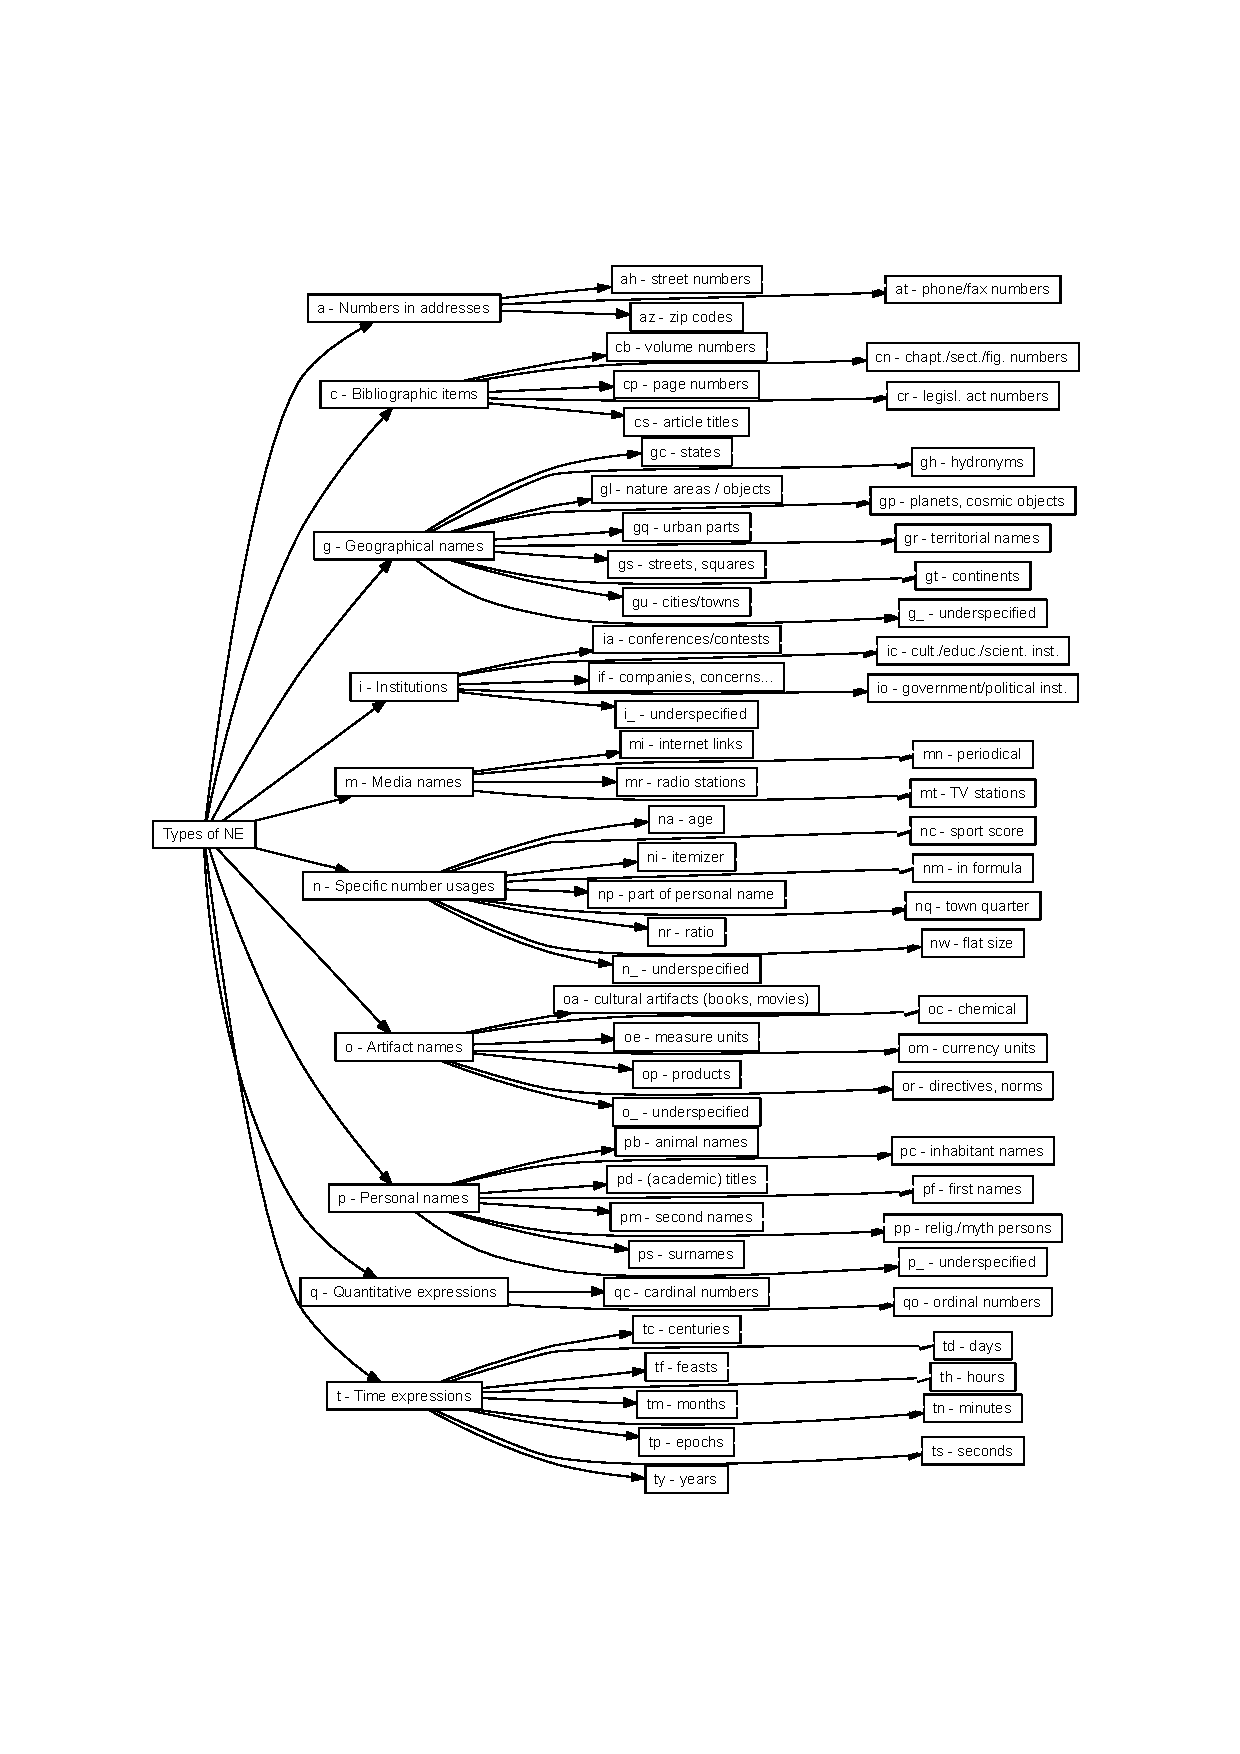
\includegraphics[width=10.5cm]{figures/core/CzechNECorpus.pdf}
	\caption{Named entity types in the Czech Named Entity corpus. Source: Czech Named Entity corpus documentation.}
	\label{fig:figures_core_CzechNECorpus}
\end{figure}


We wrote scripts that convert the XML-based format of the corpus to the format required by OpenNLP, 
manually selected the annotation types and trained the OpenNLP named entity recognizers on the resulting data.


\subsubsection*{Selecting the best approach}

Both approaches showed to have their unique advantages and disadvantages. While the first approach is 
only minimally supervised and can easily be extended to other languages that have a local version of 
Wikipedia and existing DBpedia dumps (DBpedia dumps are currently available for 97 languages\footnote{\url{http://wiki.dbpedia.org/Downloads37}}), 
our manual evaluation of the produced Named Entity recognizers showed that the 
models trained on the Czech Named Entity corpus produced better results.

More precisely, we approximated, that the DBpedia recognized far less cases and, therefore, had much lower RECALL, the PRECISION was only slightly better. We then decided, that lower RECALL is worse for our purposes -- it is better to show wrong translation to user than to not show anything.

\subsubsection*{Effectiveness}
It is worth noting that the overall effectiveness of using named entity-based retrieval was worse than we anticipated. In most subtitles, there are only few matches, but the recognition of named entities takes the most time during the data import. For this reason, we kept NE-based retrieval as a retrieval level in the core, however, we are not currently using it since the other methods already provide reasonable results and are easier to adapt to new languages and faster.

\subsection{Full-Text Search}

As another, more fuzzy level of retrieval, we use the full-text search included in \postgres. In  \postgres~full-text search, documents (in our case translation pairs) are tokenized and normalized. The result of this process is vector of normalized tokens ({\tt tsvector}). The normalization step can include lowercasing, stemming or synonyms from a dictionary and removes stop words. \postgres~builds an index over the token vector of all documents, against which queries can be run. To convert a string to a query, it is tokenized and normalized and the resulting normalized tokens are connected with an {\tt AND} operator.

The tokenization and normalization for a specific language is described in a text search configuration.\footnote{\url{http://www.postgresql.org/docs/9.1/static/textsearch-intro.html}} By default, \postgres~includes text search configurations for the following languages: Danish, Dutch, English, Finnish, French, German, Hungarian, Italian, Norwegian, Portuguese, Romanian, Russian, Spanish, Swedish, Turkish and the default ``Simple'' configuration. For Czech, a text search configuration is available from postgres.cz\footnote{\url{http://postgres.cz/wiki/Instalace_PostgreSQL}} For installation instructions, please see the technical manual in chapter~\ref{chap:technical_manual}.

When querying candidates for a Chunk, we use the {\tt ts\_rank}\footnote{\url{http://www.postgresql.org/docs/9.1/static/functions-textsearch.html}} function to pre-sort the candidates and the {\tt ts\_rank} score is later used as one of the scores in the ranking of translation pair candidates. One problem that the full-text search as a method of candidate retrieval shows, is that some of the candidates are unreasonably large documents that still have high scores because their token overlaps with the query are reasonable. We approach this problem by using our own ranking functions for translation pairs, as described in Section~\ref{sec:ranking}.


\subsection{External Services}

As another backoff level, we use Machine Translation from external services.
For this, a query with the chunk is sent to an external REST-based API. We offer a translation pair searcher for the free Machine Translation API of the MyMemory project.\footnote{ \url{http://mymemory.translated.net/doc/spec.php}} However, there is currently no machine translation service with an unlimited free API, and, for example, the MyMemory project has such a low daily quota (2500 requests/day) that the quota is quickly surpassed when translating subtitle files.

\subsection{Statistical Machine-Translation Based on Moses}
\label{sec:statmtmoses}

We tried Machine Translation first as an experiment, but it turned out the results are very good and, after some optimizations, very fast.

Moses\footnote{\url{http://www.statmt.org/moses/}} is a very popular statistical machine translation system that can work both with phrase-based models (which we use) an tree-based models (which require grammatical annotations).

We run Moses as a separate process in server mode. The sentences are sent to the Moses server through Apache's XML RPC client\footnote{It is modeled after SampleClient in Moses, \url{https://github.com/moses-smt/mosesdecoder/blob/master/contrib/server/SampleClient.java}} sentence by sentence. We have to send the sentences to Moses server already tokenized and it produces better results if the first letters of sentences are lowercased.

Because we have limited computing resources, we trained only English to Czech machine translation, since that will be most used. If we wanted to train Czech to English too, used resources would double. More information about training the machine translation and getting it to work fast can be found in Chapter~\ref{chap:moses}.

The tokenization of the input sentences, however, turned out to be problematic. Because we did not see it as a problem (since tokenization does not seem like a big problem at the first glance), we just tokenize the input with the OpenNLP tokenizers and we let Moses use its own tokenizers.

Moses, however, tokenizes English slightly different. This causes problems with the contractions of English suffixes like \texttt{-n't} and \texttt{-'ll}. For example, we tokenize \texttt{don't} as \texttt{do n't}, Moses tokenizes it as \texttt{don 't}. Those are very widely used and their wrong tokenization will, of course, produce very wrong results.

For that reason, we had to add some corrections of tokenization for the contraction suffixes -- there are not that many of them, but they are so frequent and important that we had to fix it somehow. Those corrections are hardcoded in the \texttt{MosesSearcher.scala}. This is not an ideal solution (for example, it will break with addition of a new language); more optimal solution would be to use the same tokenizers in our application and in Moses training. However, we noticed it only later, when there was no time for correction on either our database or the Moses corpus.


\section{Candidate Ranking}
\label{sec:ranking}

After retrieving candidates for a query, the candidate translation pairs must be ranked according to their quality and how well they fit the queried chunk. We use different methods for ranking the candidates retrieved by the various candidate retrieval methods. In the following section, we will briefly describe the ranking methods for each retrieval method.

All ranking methods are based on a combination of scores. Depending on the retrieval method, we assign every translation pair candidate a set of scores, which are then combined into a final score. Translation pairs are ordered by this score.

To learn the best combination of scores, we manually selected translations for heldout subtitle files and then used those annotations as positive and negative examples for training a model using the WEKA machine learning toolkit.\footnote{\url{http://www.cs.waikato.ac.nz/ml/weka/}}

\subsection{Training the Models}

For the manual annotation required to estimate weights for the scores, we started the translation memory with only the corresponding backoff level (e.g.\ exact matching or fuzzy matching) and translated heldout subtitle files using the translation workspace. After uploading and finishing the subtitle files, the class {\tt cz.filmtit.dataimport.training.GenerateTrainingset} can be used to generate a CSV file in WEKA-compatible format which can then be used to train a model.

For creating positive and negative instances, chunks without any suggestions from the translation memory are ignored. If a translation pair was selected, it is used as a positive example. If no translation pair was selected by the user, a random translation pair from the first ten suggestions is selected and used as a negative example. We select 


\subsection{Ranking for Exact Matches}

The ranking for exact matches uses a linear regression model with the following scores:

\begin{itemize}
	\item \textbf{translation pair count}\\
	The translation pair count specifies how often a translation pair has been observed. This score is calculated as $\frac{c(p)}{ \sum_{p' \in P}{c(p')}  } $\ , where $c(p)$ is the count for the translation pair $p$ and $P$ is the set of all translation pair candidates for a query.
	
	\item \textbf{source-chunk edit distance}\\
	The edit distance between the queried chunk and the source chunk of the translation pair candidate; the score is normalized by the length of the queried chunk.
	
	\item \textbf{genre match}\\
	Percentage indicting how much the genres of the queried media source overlap with the genres of the sources of the translation pair.

	\item \textbf{length difference between source and translation}\\
	The length difference between the source and target side of the translation pair candidate may indicate that an alignment is not of high quality (in most good translation pair candidates,  the length source and target side should not differ in length significantly).
	
	\item \textbf{final punctuation}\\
	Feature indicating whether the final punctuation of the queried chunk and the candidate translation match.
	
	
	
\end{itemize}



\subsection{Ranking for Full-Text Search Matches}



\begin{itemize}
	
	\item \textbf{full-text search score for the document}\\
	The score assigned by the \postgres~full text search for the document that represents the translation pair candidate.
    
	\item \textbf{translation pair count}\\
	The translation pair count specifies how often a translation pair has been observed. This score is calculated as $\frac{c(p)}{ \sum_{p' \in P}{c(p')}  } $\ , where $c(p)$ is the count for the translation pair $p$ and $P$ is the set of all translation pair candidates for a query.
	
	\item \textbf{source-chunk edit distance}\\
	The edit distance between the queried chunk and the source chunk of the translation pair candidate; the score is normalized by the length of the queried chunk.
	
	\item \textbf{genre match}\\
	Percentage indicting how much the genres of the queried media source overlap with the genres of the sources of the translation pair.

	\item \textbf{length difference between query and source}\\
	The length difference between the queried chunk and the source side of the translation pair candidate 


	\item \textbf{length difference between source and translation}\\
	The length difference between the source and target side of the translation pair candidate may indicate that an alignment is not of high quality (in most good translation pair candidates,  the length source and target side should not differ in length significantly).
	
	\item \textbf{final punctuation}\\
	Feature indicating whether the final punctuation of the queried chunk and the candidate translation match.

\end{itemize}



\section{Merging Similar Candidates}

After all translation pair candidates are retrieved and ranked on each level, we attempt to merge translation pairs that are too similar, so not to present the user with several choices that differ only very slightly.

As a translation pair merger, we currently use an implementation based on Levenshtein distance, which removes all candidates whose similarity to a higher-scoring candidate are below a given threshold (1 by default).

%TODO algorithm+analysis



\section{Technical Issues}

\subsection{Concurrency}

One important issue in the Core Translation Memory is that the service must be able to handle a large number of simultaneous requests without blocking or long delays. There are, however, some searchers, that are inherently not thread-safe.

To approach this issue, we used the Scala akka library,\footnote{\url{http://akka.io/}} which provides methods for parallelization based on the \emph{actor model}. A {\tt TranslationPairSearcherWrapper}\footnote{See  the class cz.filmtit.core.concurrency.searcher.TranslationPairSearcherWrapper.} is a {\tt TranslationPairSearcher} that is constructed with a number of other {\tt TranslationPairSearcher}s, which act as the wrapper's workers. When the {\tt TranslationPairSearcherWrapper} receives a request, it routes it to a free worker or adds it to the queue if none of the workers are free. Using this wrapper class, any non-thread-safe subclass of {\tt TranslationPairSearcher} can easily be queried in parallel.

We use the same method for parallelizing the tokenization of Chunks, since it is not thread-safe either.


\subsection{Keeping the Database Up-To-Date}

Since we want to ensure good retrieval performance, the core database is read-only in production mode. The user's translations that are stored in the User Space already are periodically added to the core database as new translation pairs and the indexes of all searchers are updated in turn.



